\documentclass[ucs]{beamer}
\usetheme{Frankfurt}
% \usecolortheme{seahorse}

\usepackage[utf8x]{inputenc}
\usepackage[T2A]{fontenc}

\usepackage[english,russian]{babel}
\usepackage{amssymb, amsmath, amsfonts, amsthm}
\usepackage{multirow}
\usepackage{booktabs}
\usepackage{array}
% \usepackage{rotating}
% \usepackage{caption}
\usepackage{pgfmath}
\usepackage{tikz}
\usetikzlibrary{arrows,fit,positioning,shapes.multipart}

\title{Верификация проекционного метода численного решения уравнения Больцмана на основе классических задач передачи тепла и массы}
\author{Рогозин Олег}
\institute{
	Московский физико-технический институт (государственный университет) \\
	Российский научный центр ``Курчатовский институт''
}

\newcommand{\dd}{\:\mathrm{d}}
\newcommand{\Kn}{\mathrm{Kn}}
\begin{document}

\frame{\titlepage}
\begin{frame}
	\frametitle{Содержание}
	\tableofcontents
\end{frame}

\section{Решение уравнения Больцмана проекционным методом}

\begin{frame}
	\frametitle{Расщепление уравнения Больцмана}
	\[
		{\partial{f} \over \partial{t}} + \boldsymbol{\xi} \cdot {\partial{f} \over \partial\mathbf{r}} = 
		\int\limits_{\mathbb R^3} \int\limits_0^{2\pi} \int\limits_0^{b_m} 
		(f_1' f' - f_1 f) gb \dd{b} \dd\varepsilon \dd\boldsymbol\xi_1
	\]
	\begin{columns}[c]
		\begin{column}{6cm}
			\begin{enumerate}
				\item уравнение переноса
				\begin{itemize}
					\item \(\displaystyle{\partial{f} \over \partial{t}} + \boldsymbol\xi \cdot {\partial{f} \over \partial\mathbf{r}} = 0\)
				\end{itemize}
				\item интеграл столкновений
				\begin{itemize}
					\item \(\displaystyle{\partial{f} \over \partial{t}} = J(f)\)
				\end{itemize}
				\item вычисление макропараметров
				\begin{itemize}
					\item \(n = \int f \dd\boldsymbol\xi$
					\item \(\mathbf{u} = \frac{1}{n}\int \boldsymbol\xi f \dd\boldsymbol\xi\)
					\item \(T = \frac{m}{3nk}\int c^2 f \dd\boldsymbol\xi\)
					\item \(P_{ij} = m \int c_i c_j f \dd\boldsymbol\xi\)
					\item \(\mathbf{q} = \frac{m}{2} \int c^2 \mathbf{c} f \dd\boldsymbol\xi\)
				\end{itemize}
			\end{enumerate}
		\end{column}
		\begin{column}{6cm}
			\centering{Симметричная схема расщепления} \\
			\bigskip
			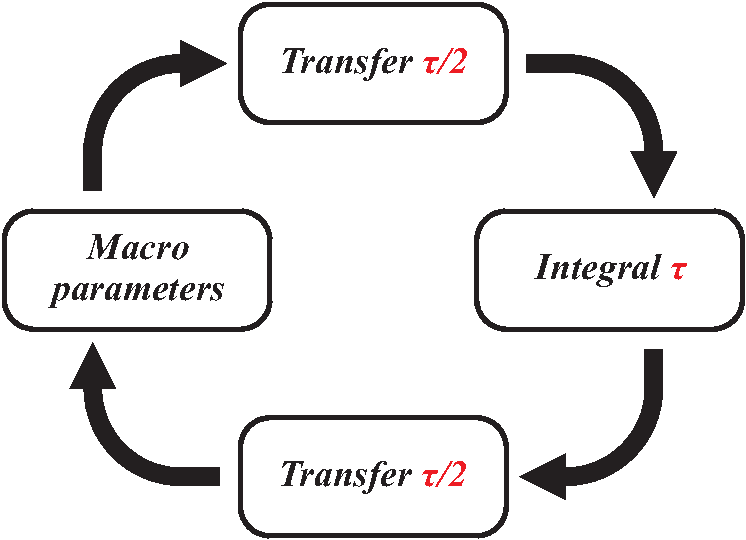
\includegraphics[width=\columnwidth]{split_scheme.pdf}
		\end{column}
	\end{columns}
\end{frame}

\begin{frame}
	\frametitle{Применяемые сетки и левая часть уравнения Больцмана}
	\begin{columns}[c]
		\column{0.5\columnwidth}
			\centering{Пространственные сетки\\}
				\smallskip
				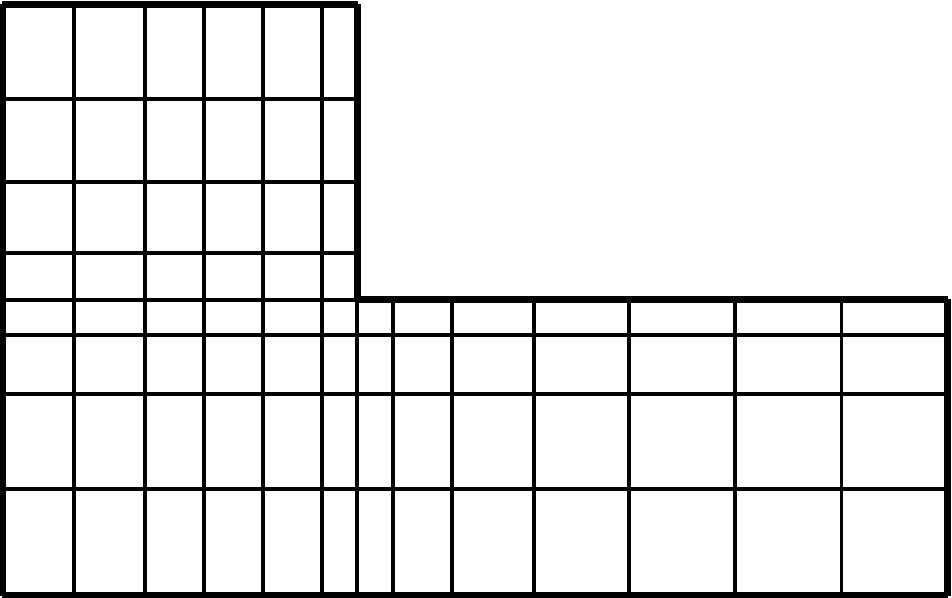
\includegraphics[width=3cm]{rectangle_mesh.pdf}\\
				\bigskip
			Консервативная TVD-схема второго порядка
		\[ {f^{j+1}_i-f^j_i \over \tau} = \xi{\tilde f_{i+1/2}-\tilde f_{i-1/2}  \over h} \]
		\[ \tilde f_{i+1/2} = f^j_i+\frac{1-\gamma}{2}\varphi(\theta) (f^j_{i+1}-f^j_i), \xi>0 \]
		\column{0.5\columnwidth}
			\centering{Скоростная сетка\\}
			\bigskip
			\begin{tikzpicture}[scale=.25]
				\foreach \x in {-10,...,10}
					\foreach \y in {-10,...,10}
					{
						\pgfmathtruncatemacro\mynumber{\x^2+\y^2}
						\ifnum \mynumber<100
							\pgfpathrectangle{\pgfpoint{\x cm}{\y cm}}{\pgfpoint{1cm}{1cm}}
						\fi
					}
				\pgfusepath{draw}
			\end{tikzpicture}
	\end{columns}
\end{frame}

\begin{frame}
	\frametitle{Правая часть уравнения Больцмана}
	\begin{itemize}
		\item симметризация интегрирование по \(\boldsymbol\xi\) и \(\boldsymbol\xi'_1\)
			\[
				J(\boldsymbol\xi_\gamma) = \int\delta(\boldsymbol\xi-\boldsymbol\xi_\gamma)
				(f_1' f' - f_1 f) gb \dd{b} \dd\varepsilon \dd\boldsymbol\xi \dd\boldsymbol\xi_1
			\]
		\item переход от интегрирования к суммированию
			\[ \int\dots\dd{b}\dd\varepsilon\dd\boldsymbol\xi\dd\boldsymbol\xi_1 \to \sum\limits_{\nu=1}^{N_\nu}\dots \]
		\item 8D интегрирующая сетка Коробова \( \{b_\nu,\varepsilon_\nu,\boldsymbol\xi_{\alpha_\nu},\boldsymbol\xi_{\beta_\nu}\} \)
	\end{itemize}
	\begin{block}{}
		\textit{Черемисин Ф.Г.} Консервативный метод вычисления интеграла столкновений Больцмана
			// Доклады РАН. — 1997. — Т. 357, № 1. — С. 53—56.
%		\textit{Tcheremissine F.G.} Solution of the Boltzmann Kinetic Equation for Low Speed Flows 
%			// Transport Theory and Statistical Physics. — 2008. — V.~37, N.~5. — P. 564—575.
	\end{block}
\end{frame}

\begin{frame}
	\frametitle{Проекционный метод}
	\begin{columns}
		\begin{column}{6cm}
			\[ 
				\boldsymbol\xi_{\alpha_\nu},\boldsymbol\xi_{\beta_\nu}\in \Omega \rightarrow
				\boldsymbol\xi'_{\alpha_\nu},\boldsymbol\xi'_{\beta_\nu}\notin \Omega 
			\]
			\begin{center}
			\begin{tikzpicture}[every node/.style={circle,draw=blue!50,fill=blue!20,thick,inner sep=0pt,minimum size=8mm}, >=latex',thick, node distance=.5]
				\node (alpha) {\footnotesize\(\boldsymbol\xi_\alpha'\)};
				\node (lambda) [below left=of alpha] {\footnotesize\(\boldsymbol\xi_\lambda\)};
				\node (lambdas) [below right=of alpha] {\footnotesize\(\boldsymbol\xi_{\lambda+s}\)};
				\draw [->] (alpha) to (lambda);
				\draw [->] (alpha) to (lambdas);
			\end{tikzpicture}
			\hspace{3mm}
			\begin{tikzpicture}[every node/.style={circle,draw=blue!50,fill=blue!20,thick,inner sep=0pt,minimum size=8mm}, >=latex',thick, node distance=.5]
				\node (beta) {\footnotesize\(\boldsymbol\xi_\beta'\)};
				\node (mu) [below left=of beta] {\footnotesize\(\boldsymbol\xi_\mu\)};
				\node (mus) [below right=of beta] {\footnotesize\(\boldsymbol\xi_{\mu-s}\)};
				\draw [->] (beta) to (mu);
				\draw [->] (beta) to (mus);
			\end{tikzpicture}
			\end{center}
		\end{column}
		\begin{column}{4cm}
			\begin{tikzpicture}[scale=.4, >=latex',thick]
				\draw[step=1, gray, very thin] (-5.4,-5.4) grid (5.4,5.4);
				\draw (0,0) circle (5);
				\draw[->] (0,0)--(4,-3) node[below right] {\footnotesize\(\boldsymbol\xi_\alpha\)};
				\draw[->] (0,0)--(-4,3) node[above left] {\footnotesize\(\boldsymbol\xi_\beta\)};
				\draw[->] (0,0)--(4.77,1.5);
				\draw[->] (0,0)--(-4.77,-1.5);
				\draw (-5,-2) circle (.1) node[anchor=north] {\footnotesize\(\boldsymbol\xi_{\lambda+s}\)};
				\draw (-4,-1) circle (.1) node[anchor=south] {\footnotesize\(\boldsymbol\xi_\lambda\)};
				\draw (5,2) circle (.1) node[anchor=south] {\footnotesize\(\boldsymbol\xi_{\mu-s}\)};
				\draw (4,1) circle (.1) node[anchor=north] {\footnotesize\(\boldsymbol\xi_\mu\)};
			\end{tikzpicture}
		\end{column}
	\end{columns}
	Регуляризация функций распределения разлетных скоростей:
	\[\left\{ \begin{array}{l l}
		\delta(\xi_{\alpha_\nu}'-\xi_\gamma) = (1-{\color{blue}r_\nu}) \delta(\xi_{\lambda_\nu} - \xi_\gamma) + {\color{blue}r_\nu} \delta(\xi_{\lambda_\nu+s} - \xi_\gamma)  \\
		\delta(\xi_{\beta_\nu}'-\xi_\gamma) = (1-{\color{blue}r_\nu}) \delta(\xi_{\mu_\nu} - \xi_\gamma) + {\color{blue}r_\nu} \delta(\xi_{\mu_\nu-s} - \xi_\gamma)  \\
	\end{array}\right. \]
	\[(\xi_{\alpha_\nu}') ^ 2 + (\xi_{\beta_\nu}') ^2 = (1 - {\color{blue}r_\nu}) (\xi_{\lambda_\nu} ^ 2 + \xi_{\mu_\nu} ^2) +
	{\color{blue}r_\nu} (\xi_{\lambda_\nu+s} ^ 2 + \xi_{\mu_\nu-s} ^2)\]
	\[f_{\alpha_\nu}' f_{\beta_\nu}' = (f_{\lambda_\nu} f_{\mu_\nu})^{1 - {\color{blue}r_\nu}} + (f_{\lambda_\nu+s} f_{\mu_\nu-s})^{{\color{blue}r_\nu}}\]
\end{frame}

\section{Задача теплопроводности}
\begin{frame}
	\frametitle{Постановка задачи}
	\begin{itemize}
		\item 1D задача переноса тепла между параллельными пластинами \\
		\item линейная \(T_1-T_2 \ll T_1+T_2\) \\
		\item безразмерный поток тепла \(q/(p_0\nu_0 \frac{T_1-T_2}{T_1+T_2})\) \\
		\item от числа Кнудсена \(\mathrm{Kn} = \ell_0/L\) \\
	\end{itemize}
\end{frame}

\begin{frame}
	\frametitle{Сравнение результатов}
	\begin{center}
		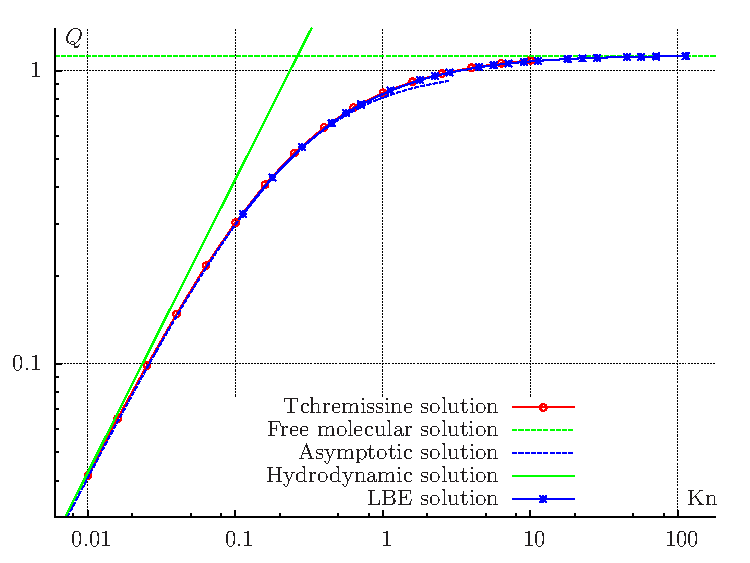
\includegraphics[width=.9\textwidth]{pics/heat.pdf}
	\end{center}
\end{frame}

\section{Течение Пуазёйля}

\begin{frame}
	\frametitle{История решения задачи Пуазёйля}
	\begin{itemize}
		\item \textit{James Maxwell, 1879} \\ формулировка условий скольжения газа вдоль стенок \\
		\item \textit{Martin Knudsen, 1909} \\ экспериментальное определение минимума потока газа \\
		\item \textit{Carlo Cercignani, 1963} \\ первое численное решение на основе кинетического уравнения БГК \\
		\item \textit{Taku Ohwada, Yoshio Sone, Kazuo Aoki, 1989} \\ точное решение задачи для модели твёрдых сфер \\
	\end{itemize}
\end{frame}

\begin{frame}
	\frametitle{Постановка задачи}
	\centering
	\begin{tikzpicture}[dashdot/.style={dash pattern=on .4pt off 3pt on 4pt off 3pt},
						>=latex',thick, scale=1]
		\fill[gray!20] (0,0) -- (3.6,0) -- (3.6,1) -- (0,1) -- cycle;
		\draw[dashdot] (-.2,0) -- (3.8,0);
		\draw[very thick] (0,1) -- (1.8,1) node[above] {\(T_0\)} -- (3.6,1);
		\draw[<->] (.7,0) -- (.7,.5) node[left] {\(\dfrac{L}{2}\)} -- (.7,1);
		\draw[<->] (3.2,0) node[above] {\(z\)} -- (2.4,0) -- (2.4,.8) node[right] {\(x\)};
	\end{tikzpicture}\\
	\bigskip
	\begin{itemize}
		\item 1D задача течения газа между параллельными пластинами \\
		\item линейная \(\left|\frac{\partial p}{\partial z}\right| \ll \frac{p}{L} \) \\
		\item безразмерный поток массы \(Q/(2p_z L^2/\nu_0)\) \\
	\end{itemize}
\end{frame}

\begin{frame}
	\frametitle{Сравнение результатов}
	\begin{center}
		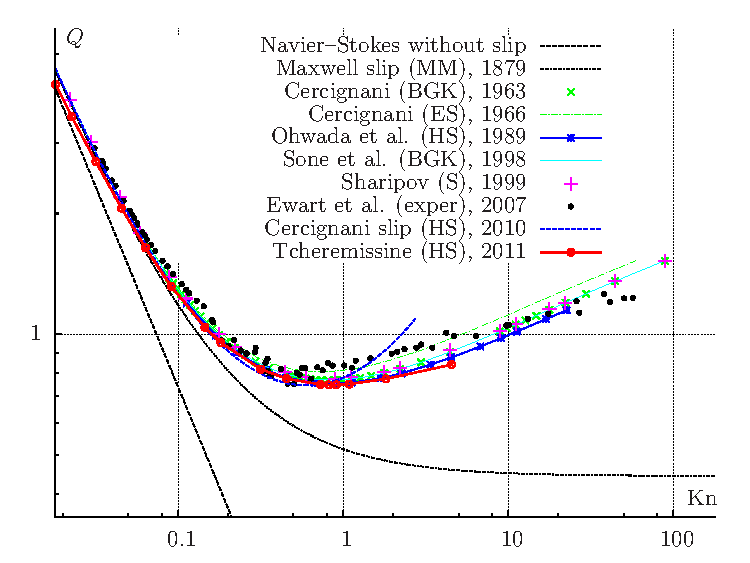
\includegraphics[width=.9\textwidth]{pics/poise.pdf}
	\end{center}
\end{frame}

\section*{}
\begin{frame}
	\frametitle{Заключение}
	На основе решения изложенных задач о медленных течениях разреженного газа можно заключить:
	\begin{itemize}
		\item Проекционный метод обеспечивает высокую точность решения в произвольной геометрии \\
		\item Легко обобщается для нелинейных задач \\
		\item Невысокие требования к вычислительным ресурсам (по сравнению с DSMC) \\
	\end{itemize}
	Среди недостатков следует выделить:
	\begin{itemize}
		\item Сложность оценки точности и достоверности полученных результатов \\
		\item Процентные отклонения от коэффициентов вязкости и теплопроводности \\
	\end{itemize}
\end{frame}

\end{document}
